% Appendix A

\chapter{Figuras} % Main appendix title

\label{AppendixA} % For referencing this appendix elsewhere, use \ref{AppendixA}

\begin{figure}[ht]
        \centering
        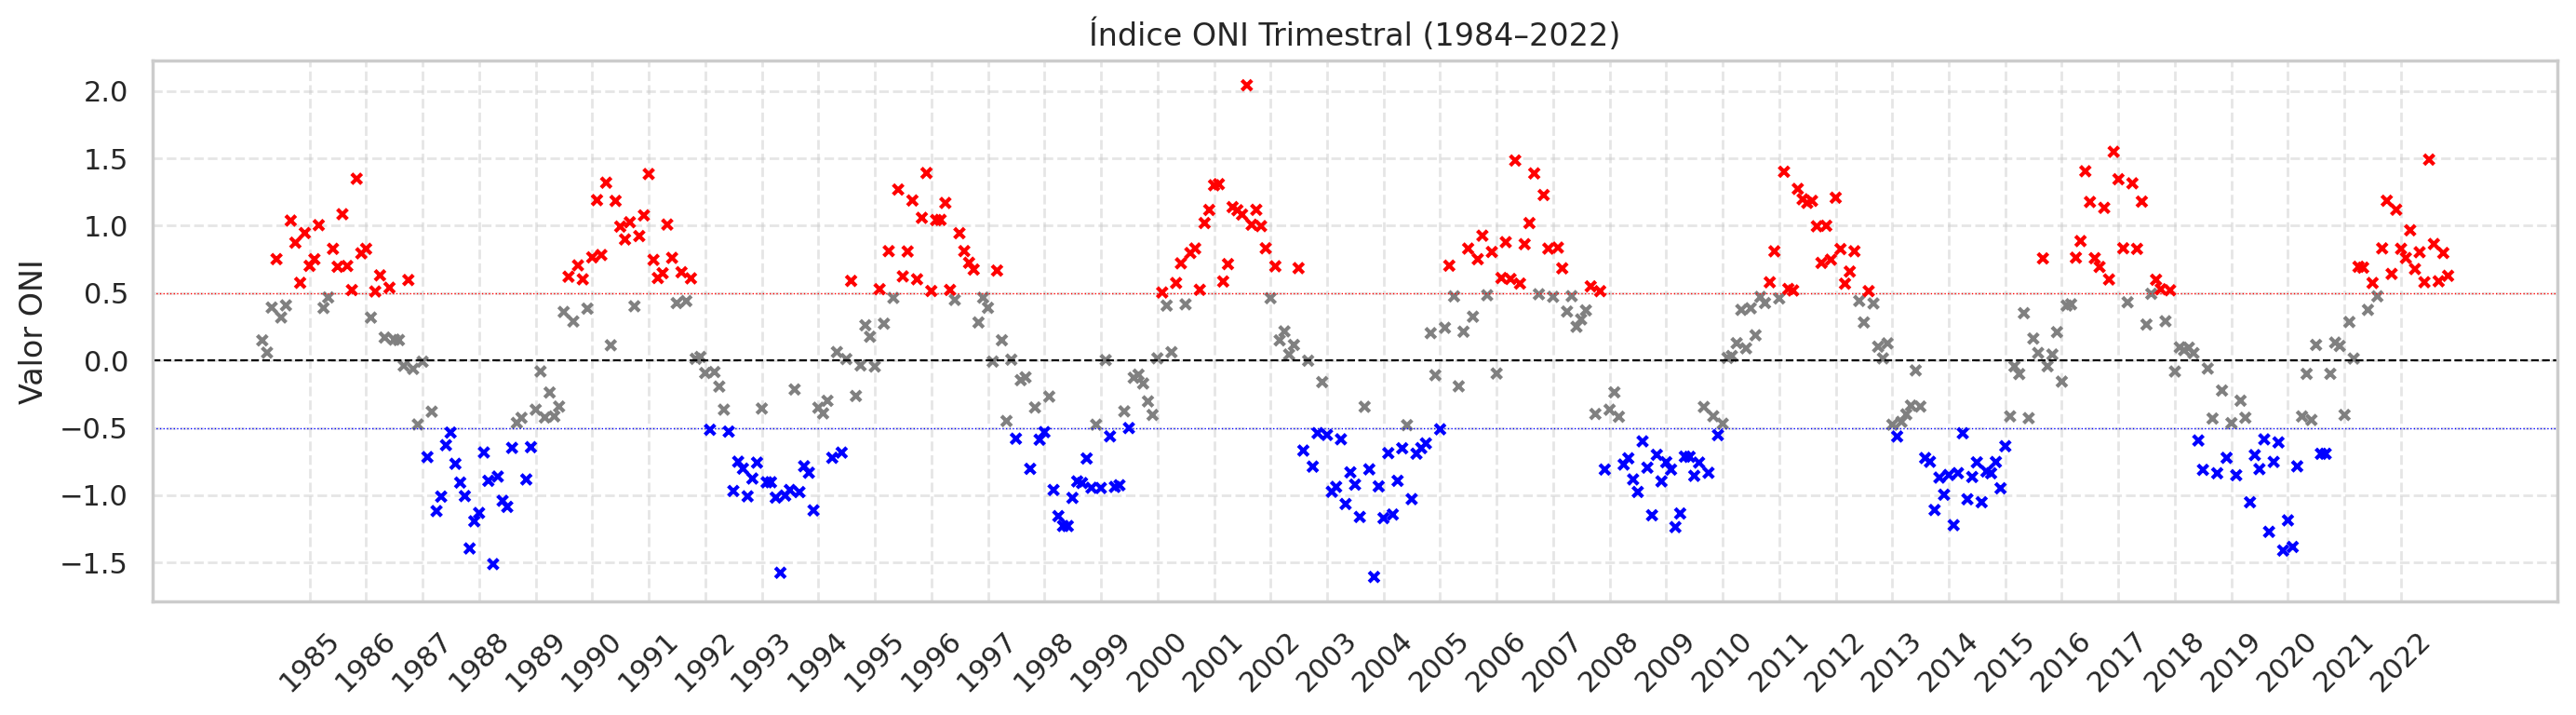
\includegraphics[scale=.38]
        {Figures/fig13_oni.png}
        \caption{Índice ONI (1984-2022).}
        \label{fig:indice_oni}
\end{figure}

\begin{figure}[ht]
        \centering
        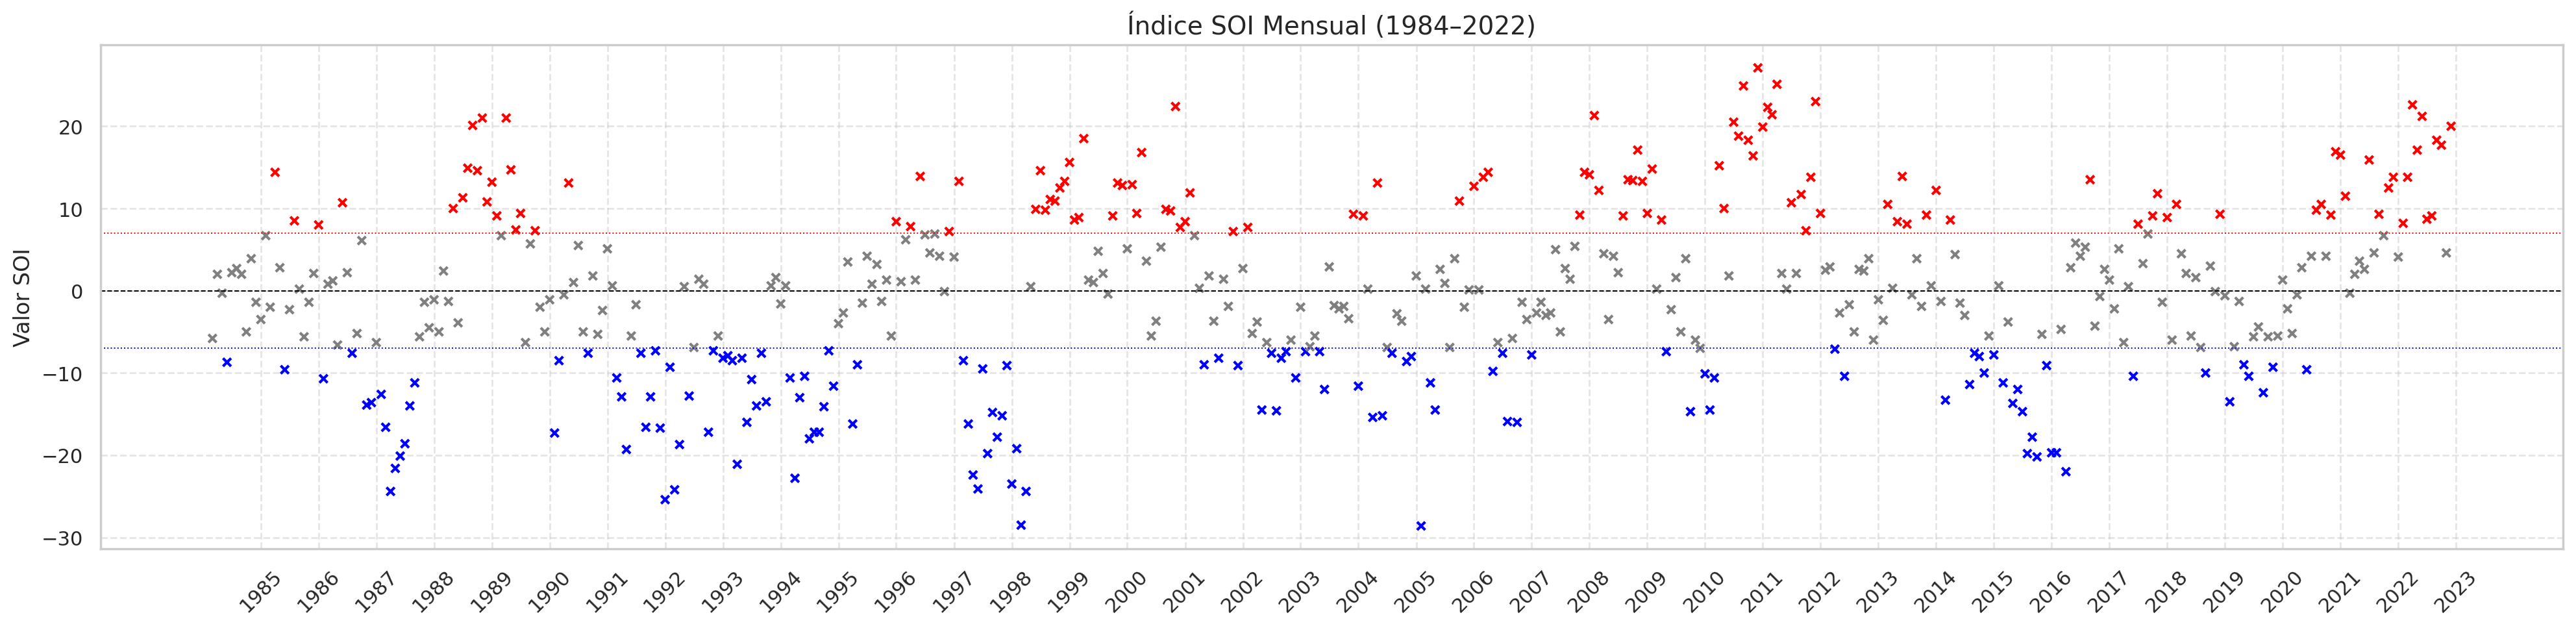
\includegraphics[scale=.26]
        {Figures/fig14_soi.png}
        \caption{Índice SOI (1984-2022).}
        \label{fig:indice_soi}
\end{figure}

\begin{figure}[ht]
        \centering
        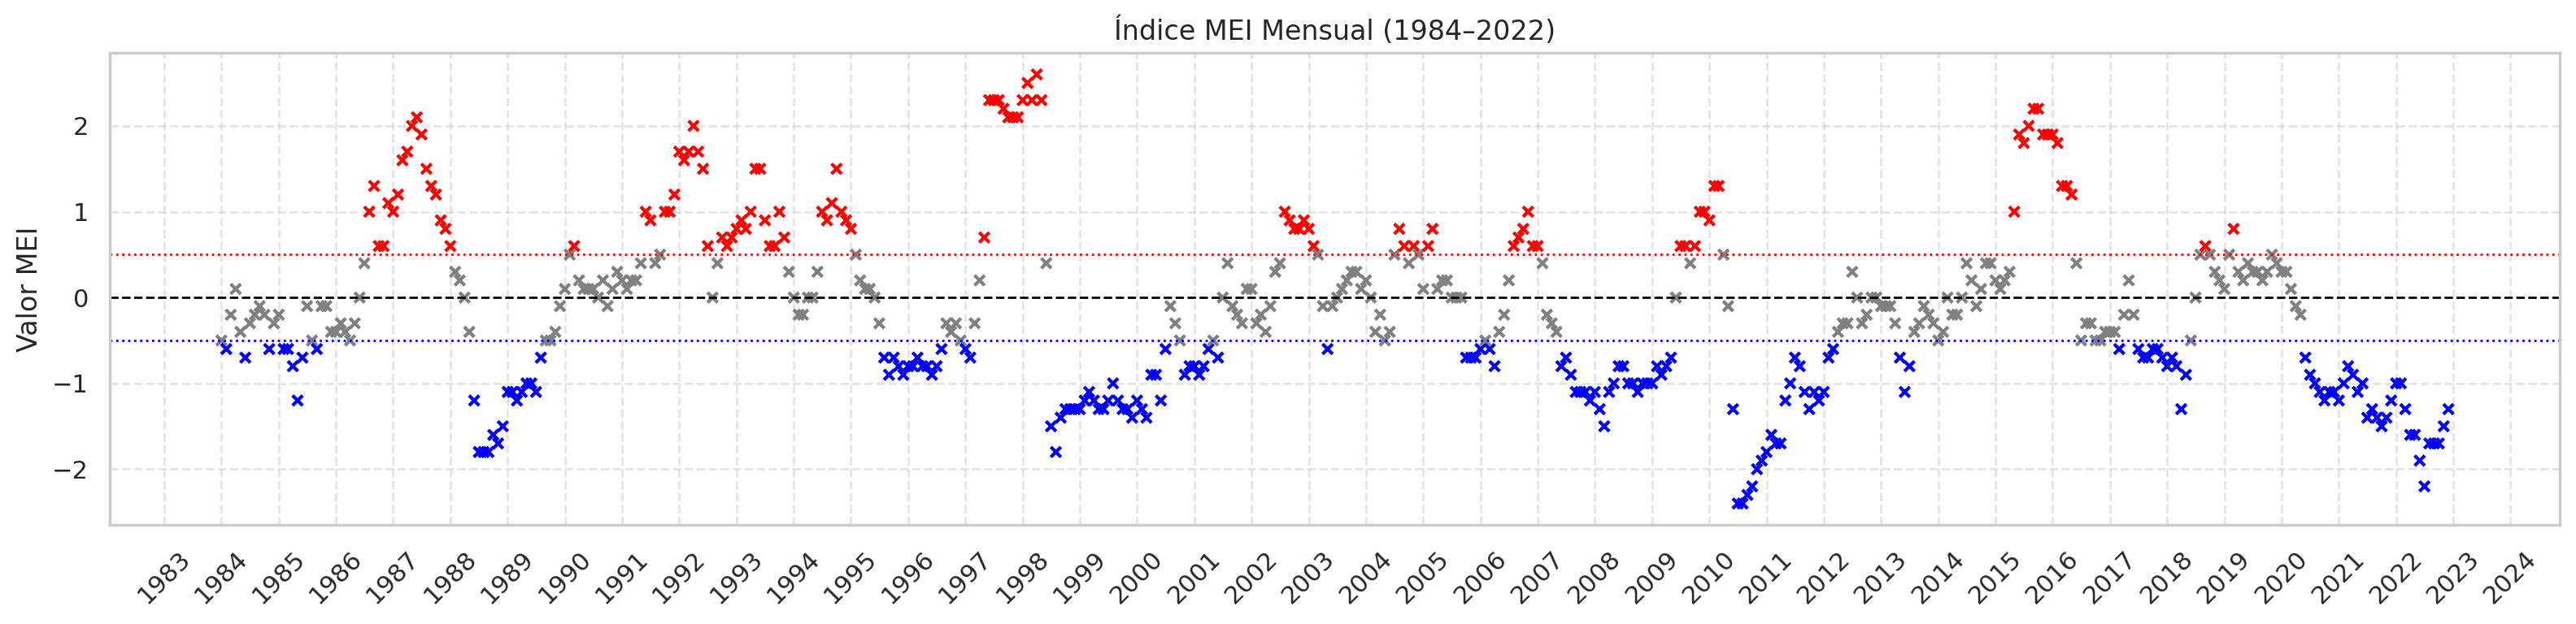
\includegraphics[scale=.32]
        {Figures/fig15_mei.png}
        \caption{Índice MEI (1984-2022).}
        \label{fig:indice_mei}
\end{figure}

\begin{figure}[ht]
        \centering
        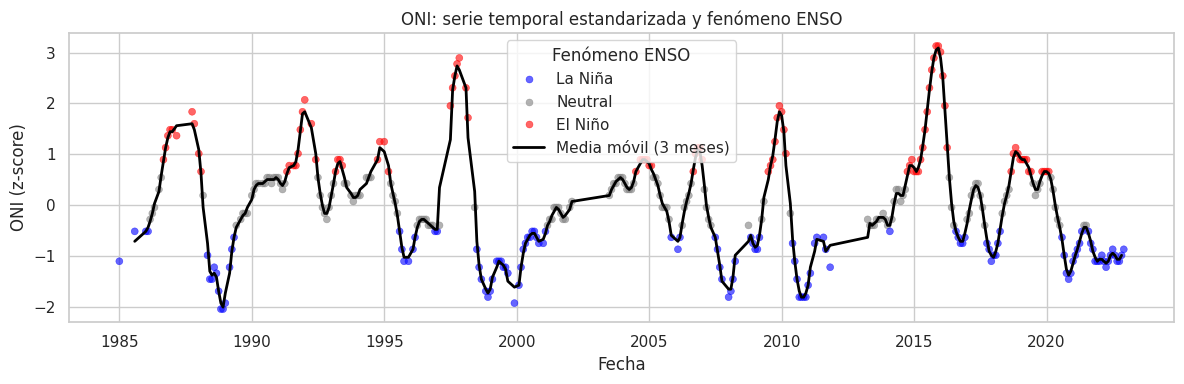
\includegraphics[scale=.45]
        {Figures/fig17_ts_oni.png}
        \caption{Índice ONI (1984-2022).}
        \label{fig:indice_oni_ts}
\end{figure}

\begin{figure}[ht]
        \centering
        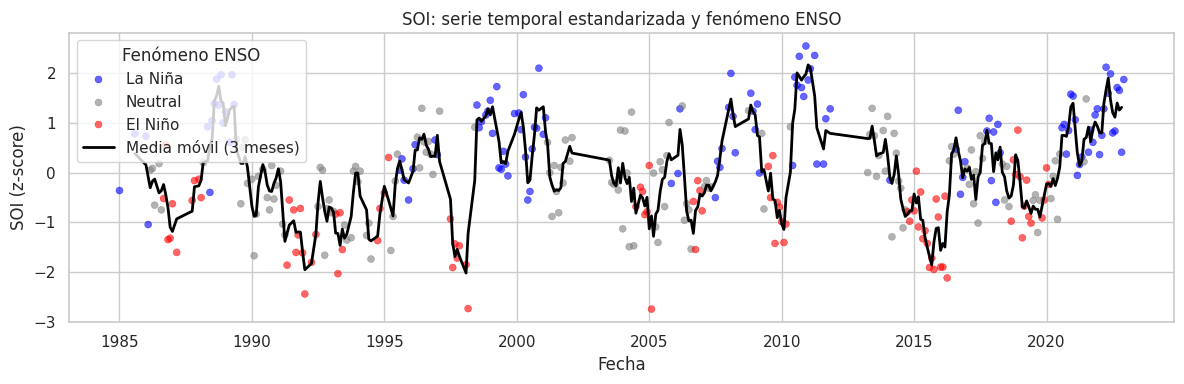
\includegraphics[scale=.45]
        {Figures/fig18_ts_soi.png}
        \caption{Índice SOI (1984-2022).}
        \label{fig:indice_soi_ts}
\end{figure}

\begin{figure}[ht]
        \centering
        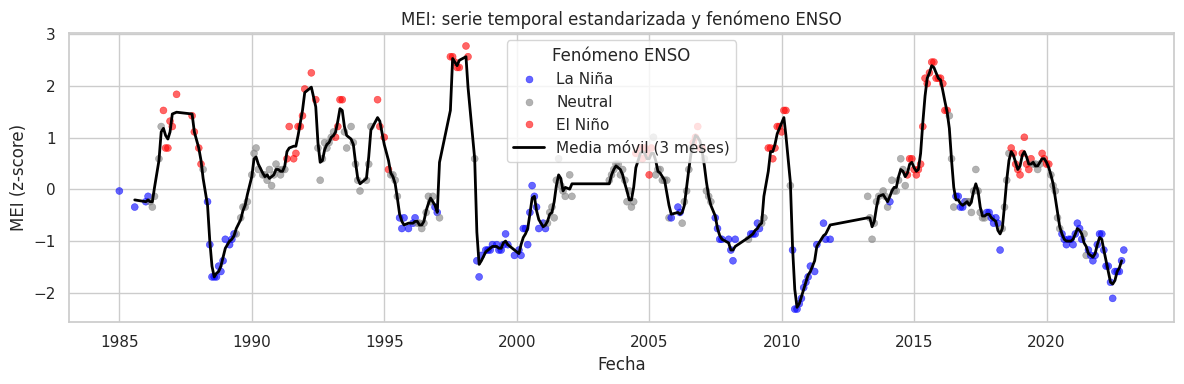
\includegraphics[scale=.45]
        {Figures/fig19_ts_mei.png}
        \caption{Índice MEI (1984-2022).}
        \label{fig:indice_mei_ts}
\end{figure}

\begin{figure}[htpb]
    \centering
    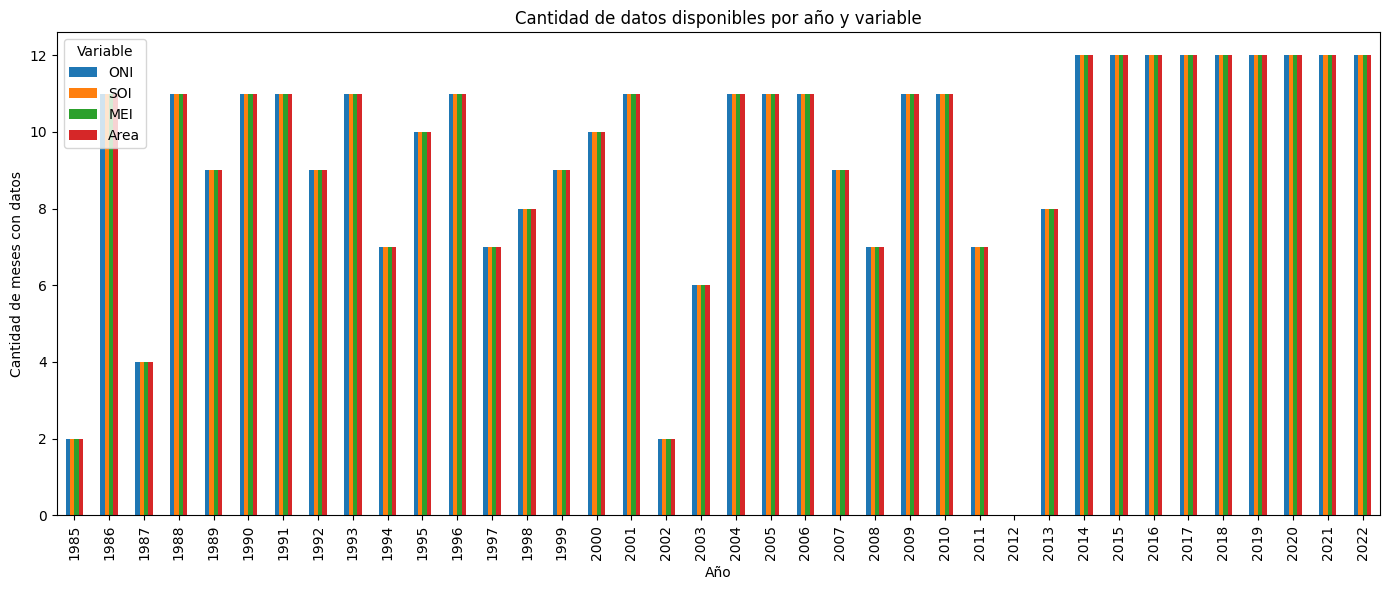
\includegraphics[scale=.40]{Figures/conteo_series.png}
    \caption{Cantidad de meses con datos disponibles por año y variable (ONI, SOI, MEI, Área).}
    \label{fig:conteo_datos}
\end{figure}

\begin{figure}[H]
    \centering
    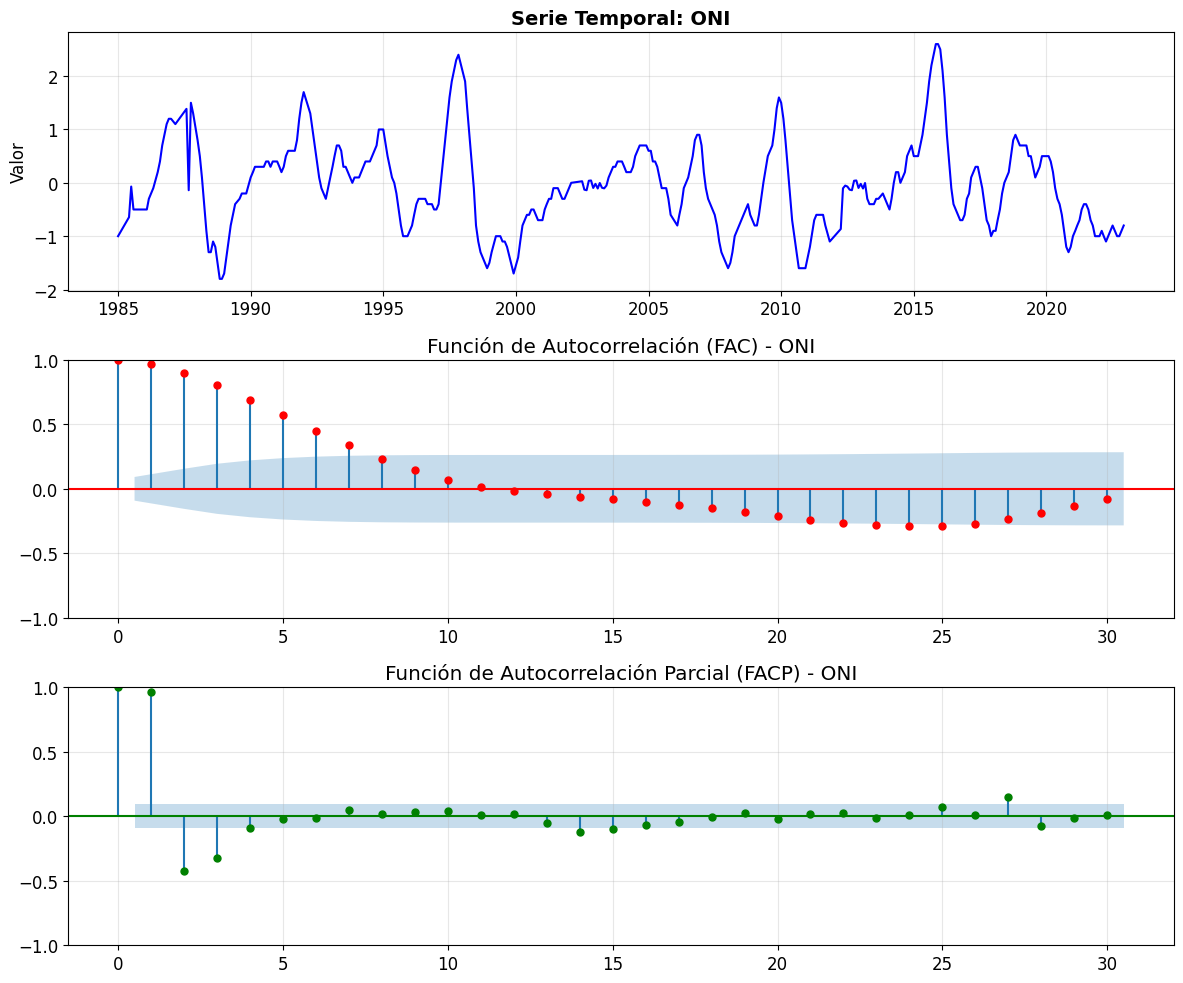
\includegraphics[scale=.42]{Figures/facp_ONI.png}
    %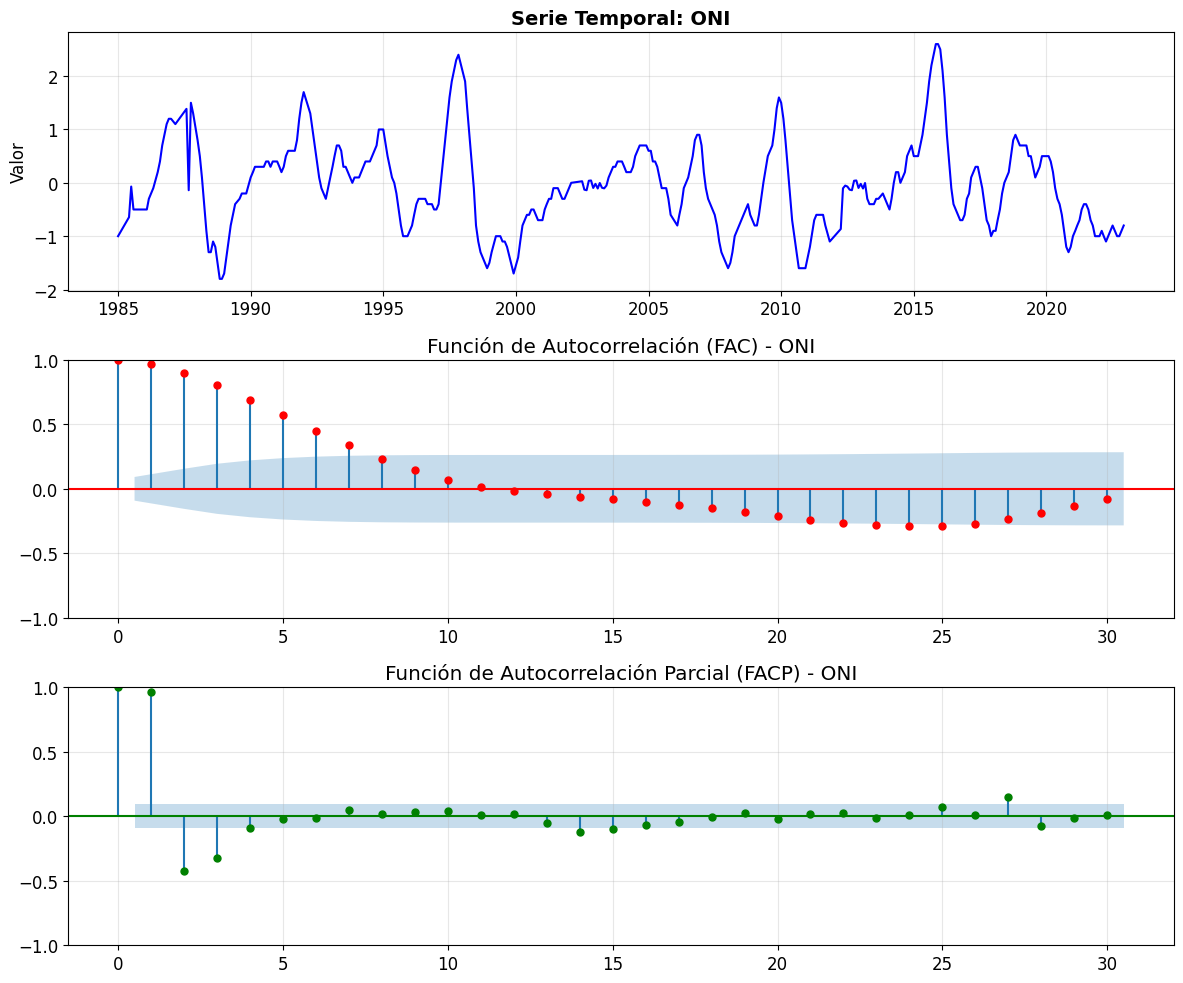
\includegraphics[width=0.7\textwidth]{Figures/facp_ONI.png}
    \caption{Funciones ACF y PACF de la serie ONI.}
    \label{fig:facp_oni}
\end{figure}

\begin{figure}[H]
    \centering
    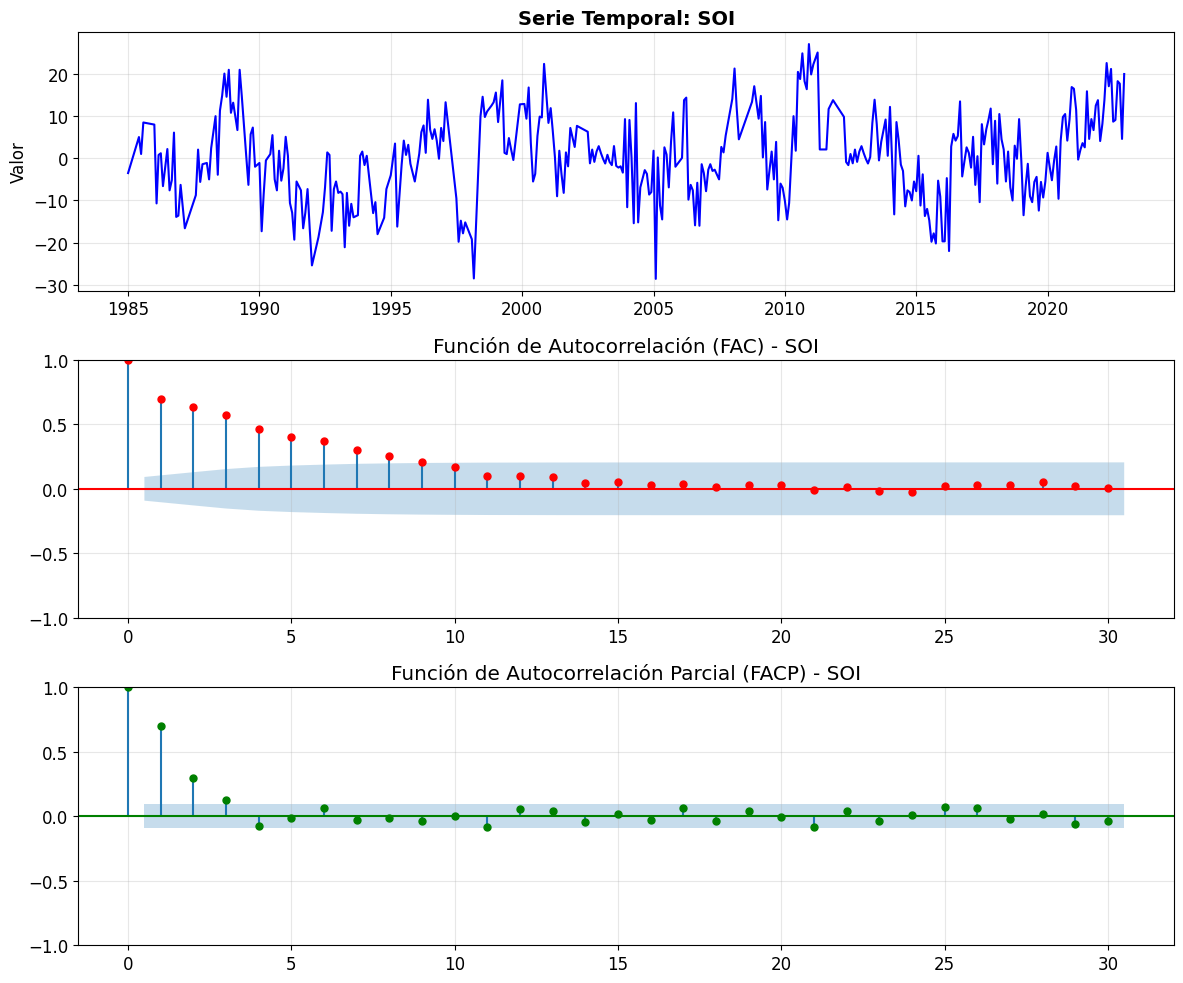
\includegraphics[scale=.42]{Figures/facp_SOI.png}
    \caption{Funciones ACF y PACF de la serie SOI.}
    \label{fig:facp_soi}
\end{figure}

\begin{figure}[H]
    \centering
    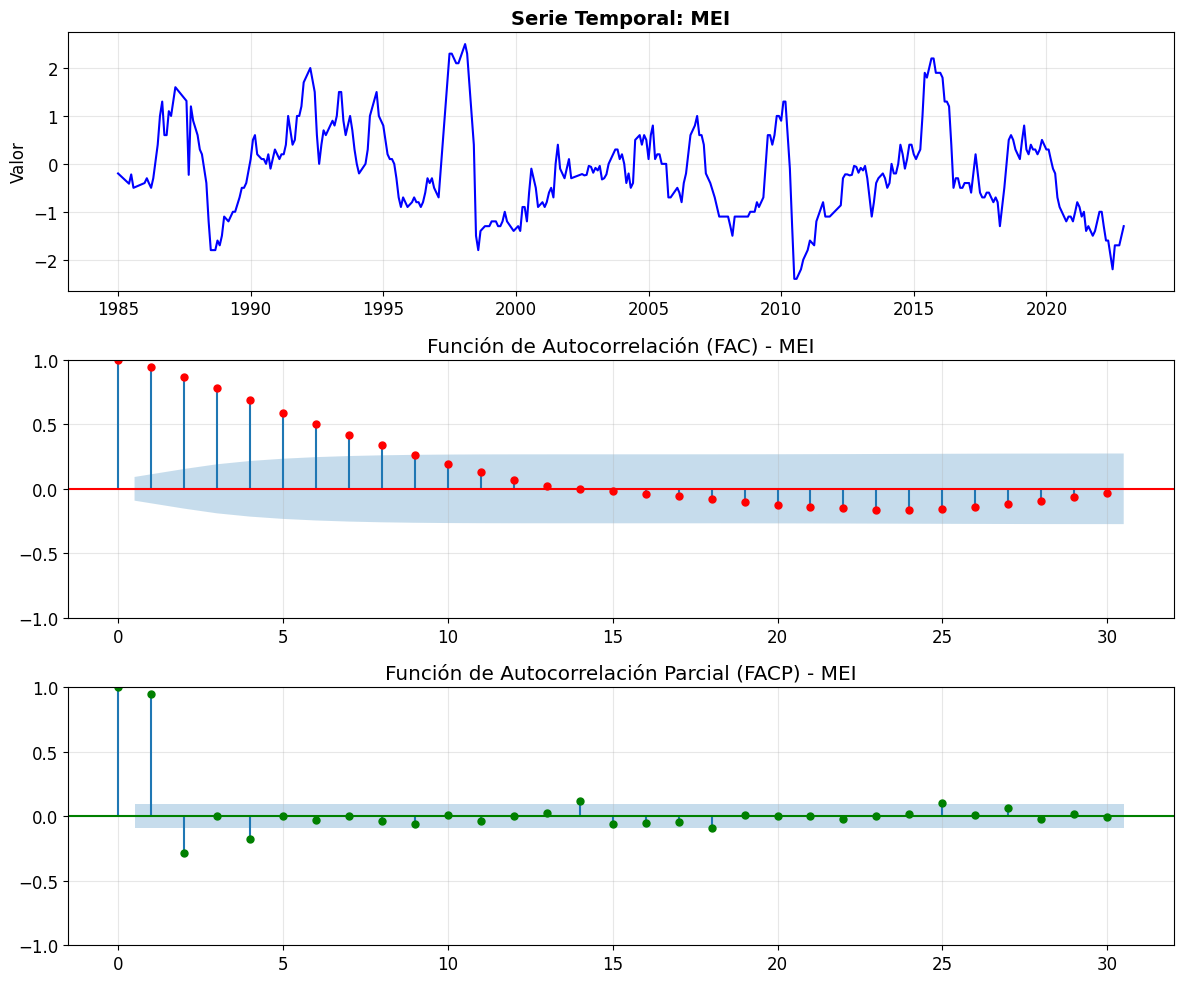
\includegraphics[scale=.42]{Figures/facp_MEI.png}
    \caption{Funciones ACF y PACF de la serie MEI.}
    \label{fig:facp_mei}
\end{figure}

\begin{figure}[H]
    \centering
    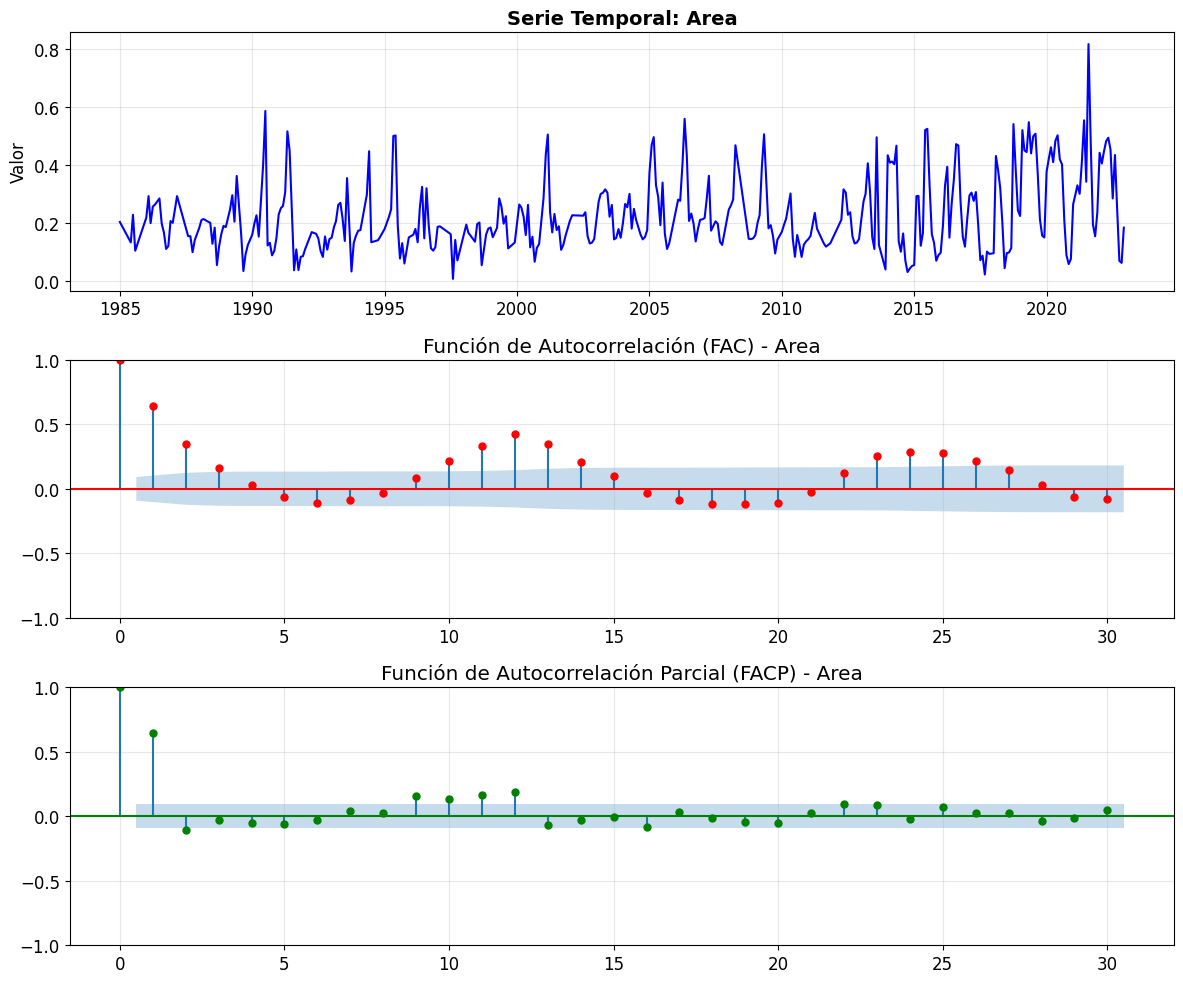
\includegraphics[scale=.42]{Figures/facp_Area.png}
    \caption{Funciones ACF y PACF de la serie Área (superficie de agua).}
    \label{fig:facp_area}
\end{figure}


\begin{figure}[H]\centering
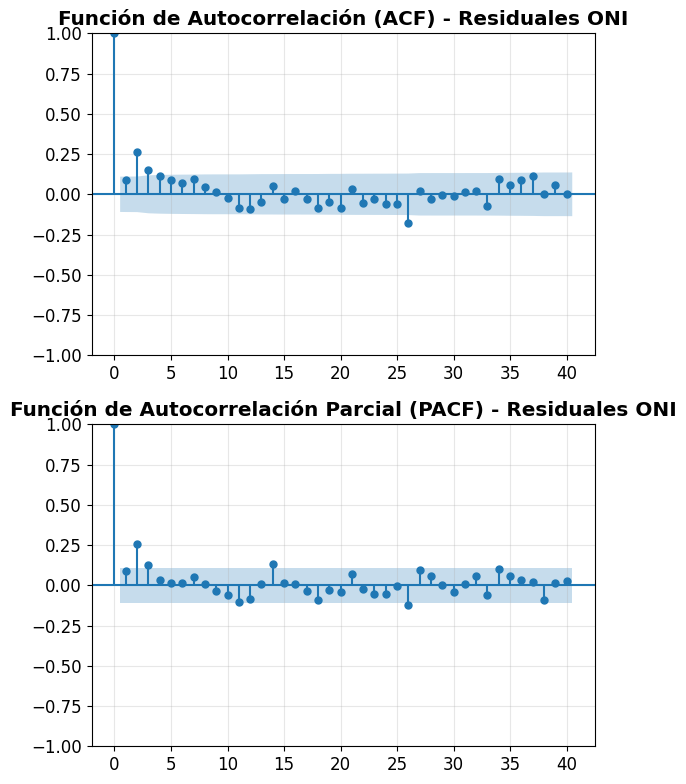
\includegraphics[scale=.52]{Figures/acf_pacf_res_oni.png}
\caption{ONI: ACF y PACF de los residuos.}
\label{fig:acf_pacf_res_oni}
\end{figure}

\begin{figure}[H]\centering
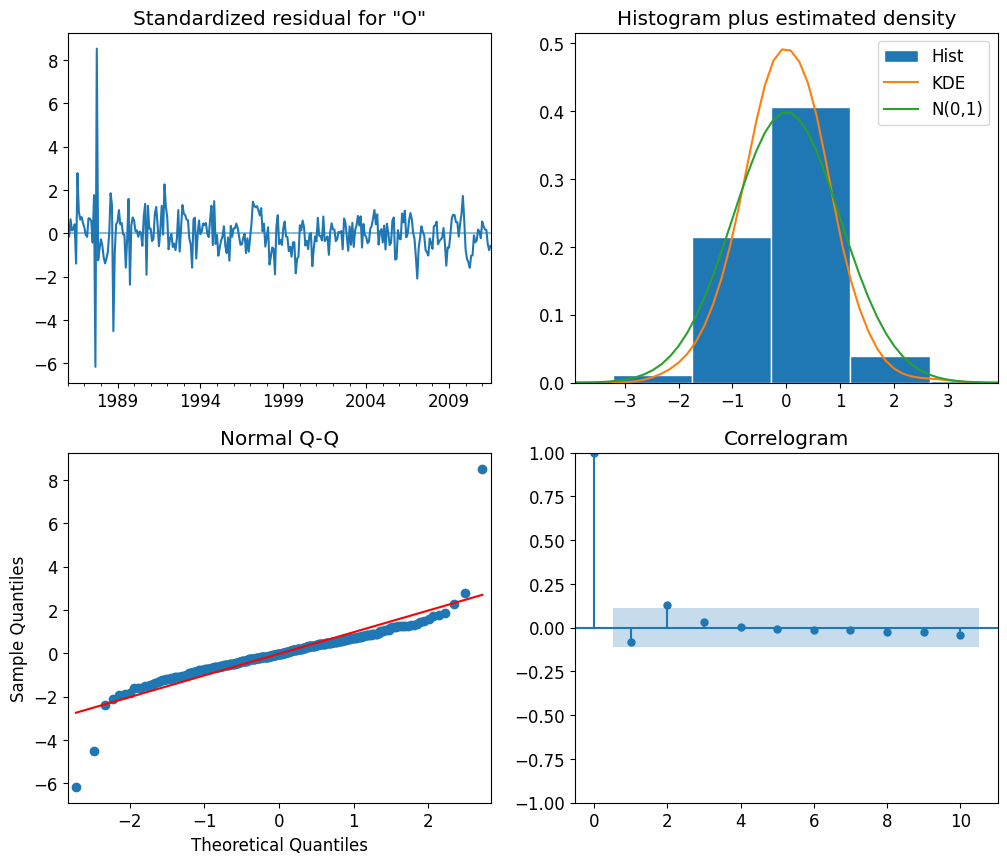
\includegraphics[scale=.52]{Figures/res_std_oni.png}
\caption{ONI: diagnóstico estándar de residuos (histograma, densidad, Q--Q, correlograma).}
\label{fig:std_oni}
\end{figure}

\begin{figure}[H]\centering
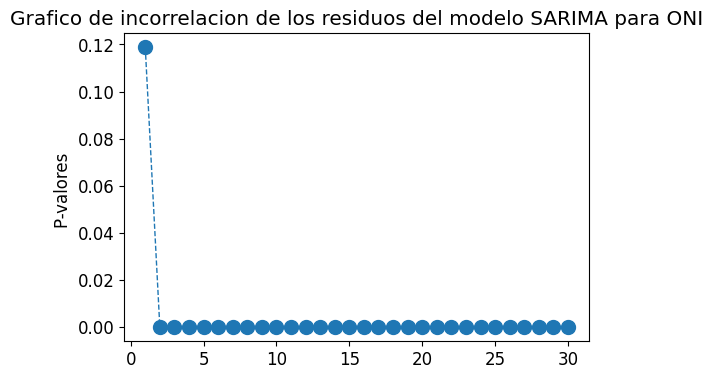
\includegraphics[scale=.52]{Figures/inco_oni.png}
\caption{ONI: gráfico de incorrelación (p--valores Ljung--Box por lag).}
\label{fig:inco_oni}
\end{figure}


\begin{figure}[H]\centering
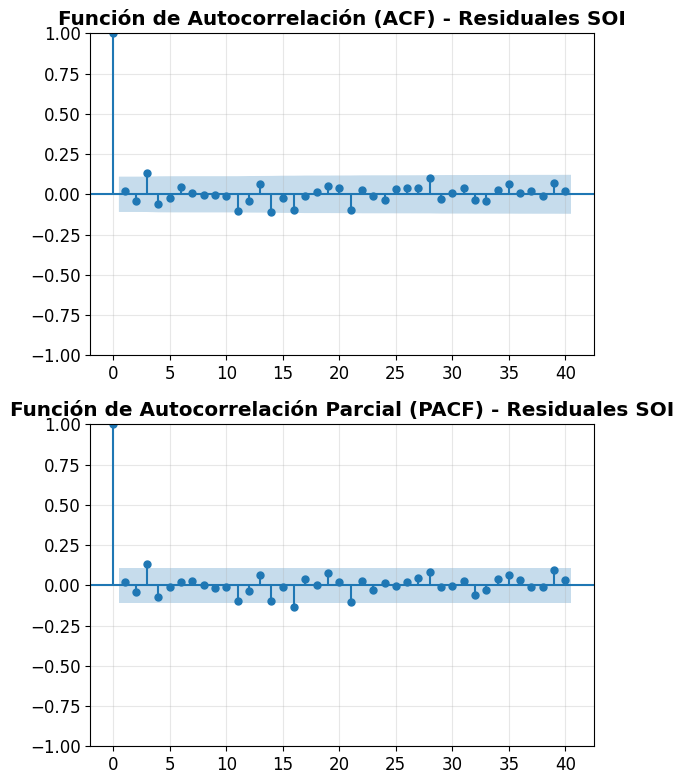
\includegraphics[scale=.52]{Figures/acp_pacf_res_soi.png}
\caption{SOI: ACF y PACF de los residuos.}
\label{fig:acf_pacf_res_soi}
\end{figure}

\begin{figure}[H]\centering
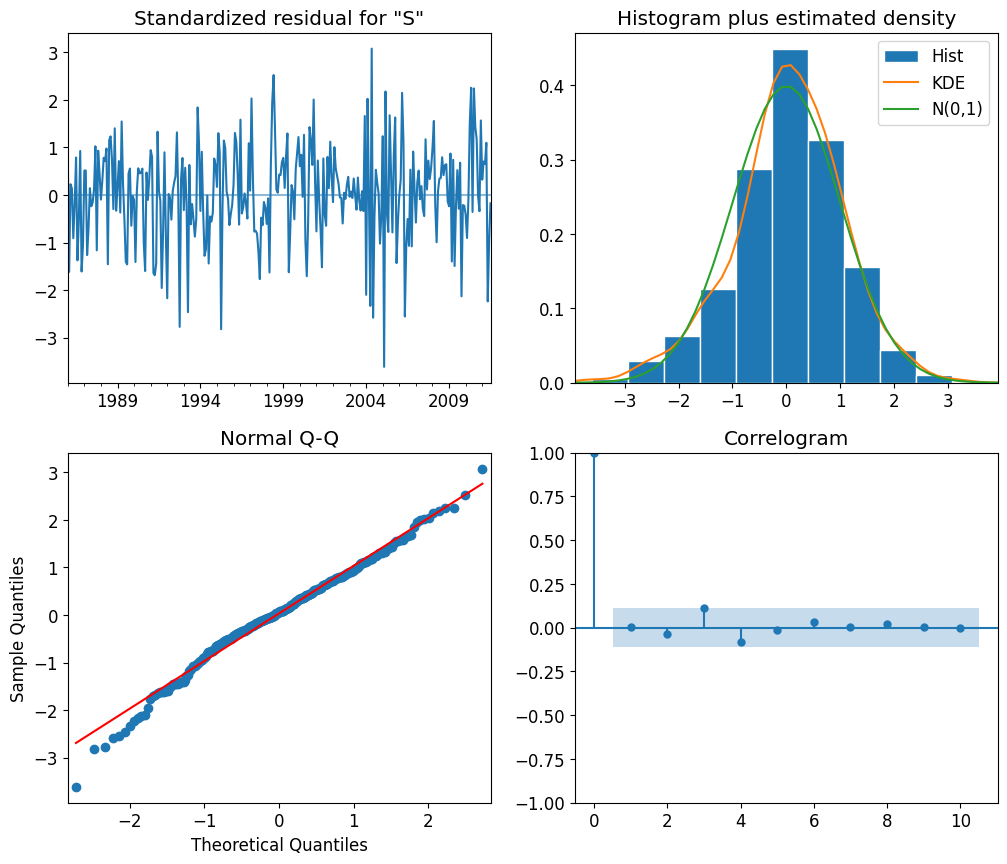
\includegraphics[scale=.52]{Figures/res_std_soi.png}
\caption{SOI: diagnóstico estándar de residuos (histograma, densidad, Q--Q, correlograma).}
\label{fig:std_soi}
\end{figure}

\begin{figure}[H]\centering
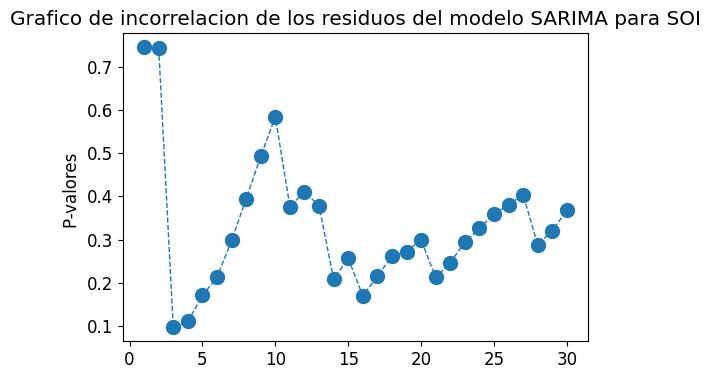
\includegraphics[scale=.52]{Figures/inco_soi.png}
\caption{SOI: gráfico de incorrelación (p--valores Ljung--Box por lag).}
\label{fig:inco_soi}
\end{figure}



\begin{figure}[H]\centering
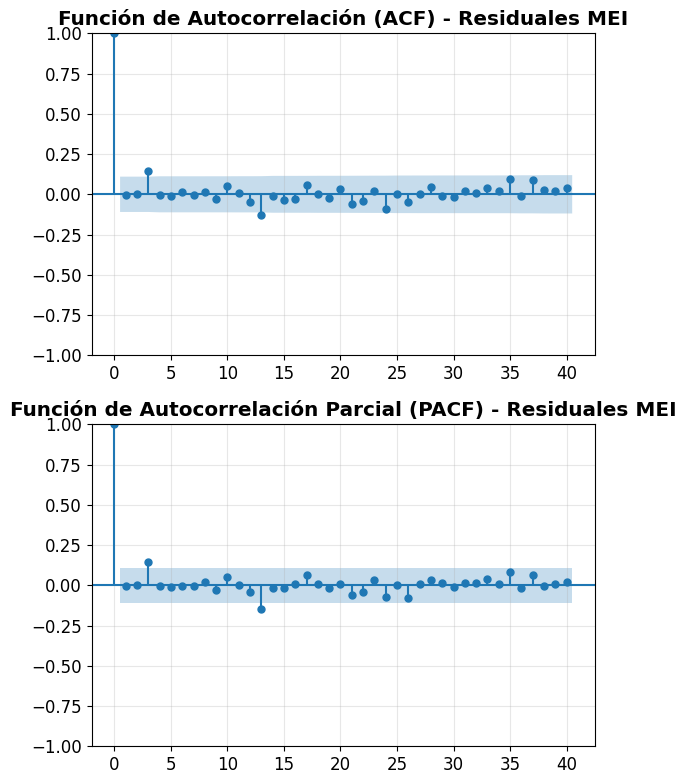
\includegraphics[scale=.52]{Figures/acf_pacf_res_mei.png}
\caption{MEI: ACF y PACF de los residuos.}
\label{fig:acf_pacf_res_mei}
\end{figure}

\begin{figure}[H]\centering
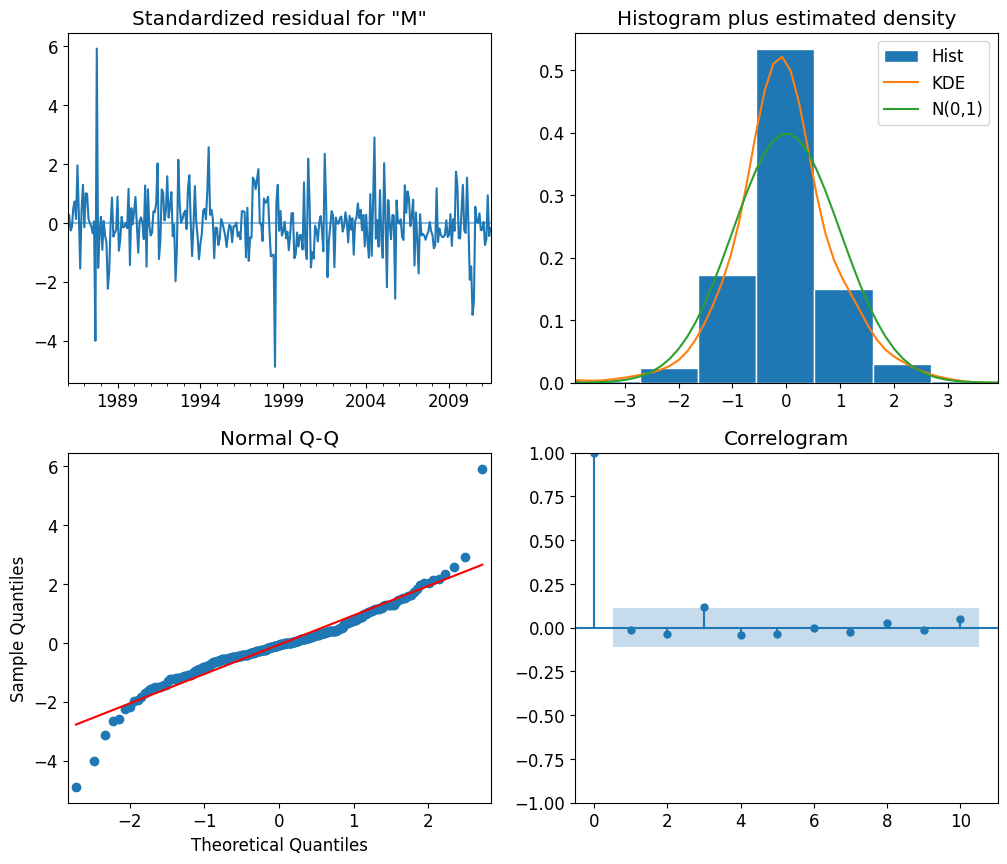
\includegraphics[scale=.52]{Figures/res_std_mei.png}
\caption{MEI: diagnóstico estándar de residuos (histograma, densidad, Q--Q, correlograma).}
\label{fig:std_mei}
\end{figure}

\begin{figure}[H]\centering
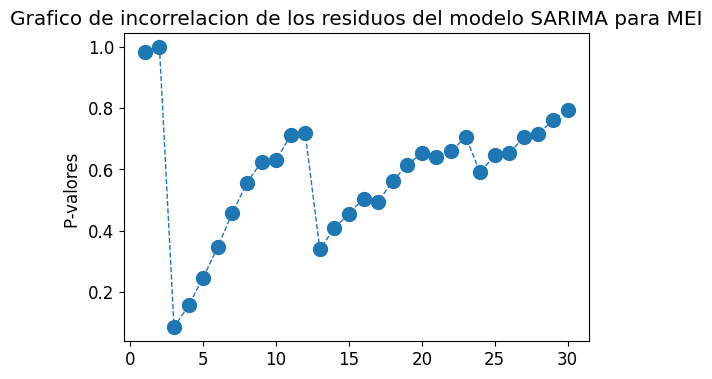
\includegraphics[scale=.52]{Figures/inco_mei.png}
\caption{MEI: gráfico de incorrelación (p--valores Ljung--Box por lag).}
\label{fig:inco_mei}
\end{figure}

\begin{figure}[H]\centering
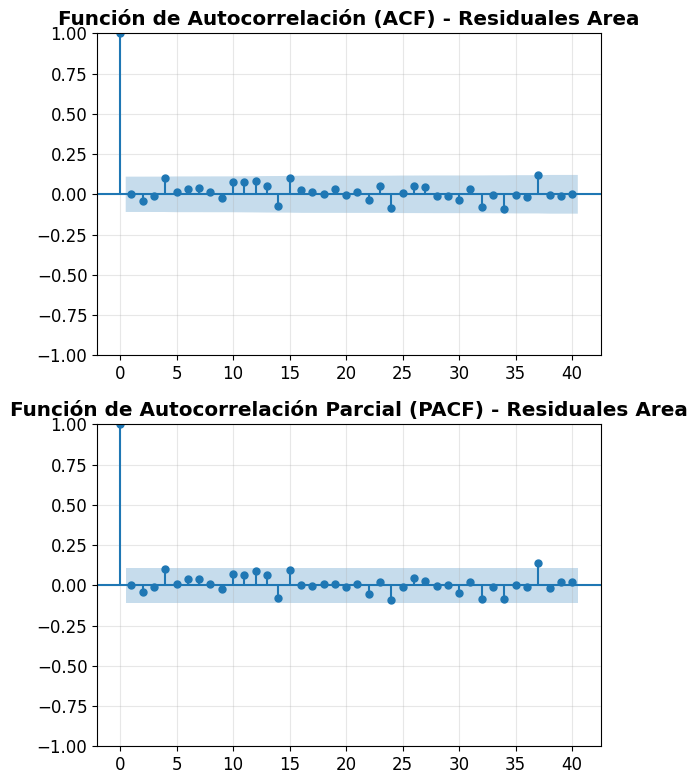
\includegraphics[scale=.52]{Figures/acf_pacf_res_area.png}
\caption{Área: ACF y PACF de los residuos.}
\label{fig:acf_pacf_res_area}
\end{figure}

\begin{figure}[H]\centering
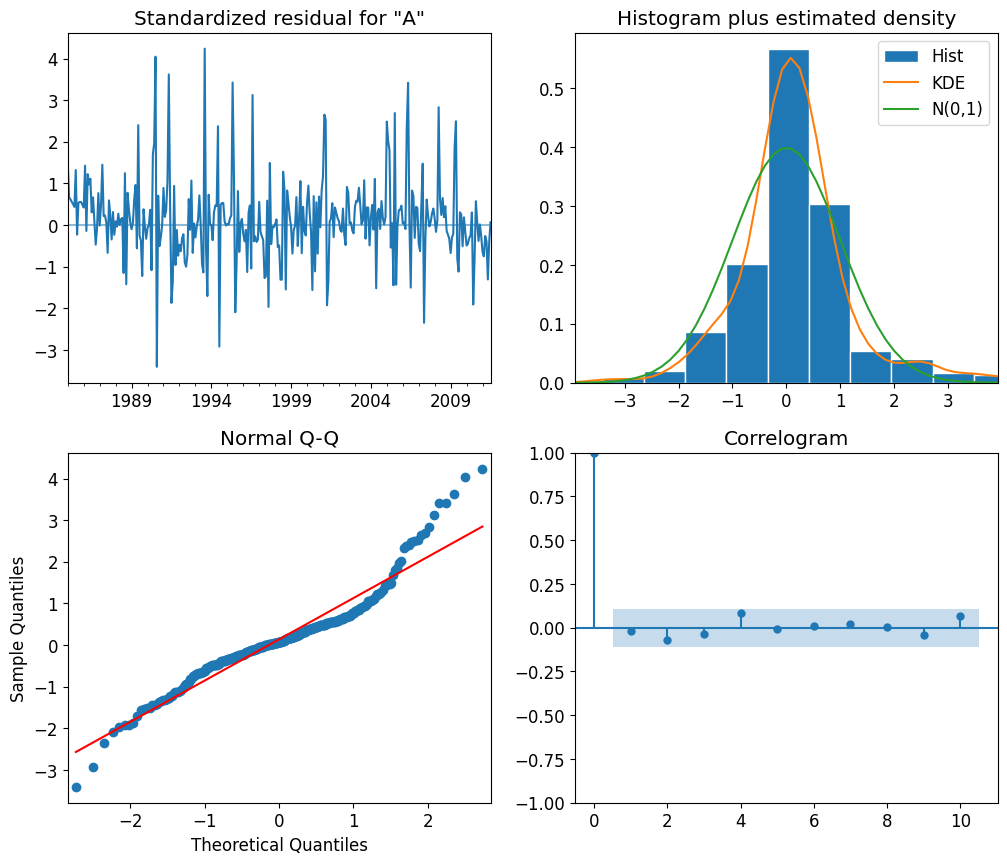
\includegraphics[scale=.52]{Figures/res_std_area.png}
\caption{Área: diagnóstico estándar de residuos (histograma, densidad, Q--Q, correlograma).}
\label{fig:std_area}
\end{figure}

\begin{figure}[H]\centering
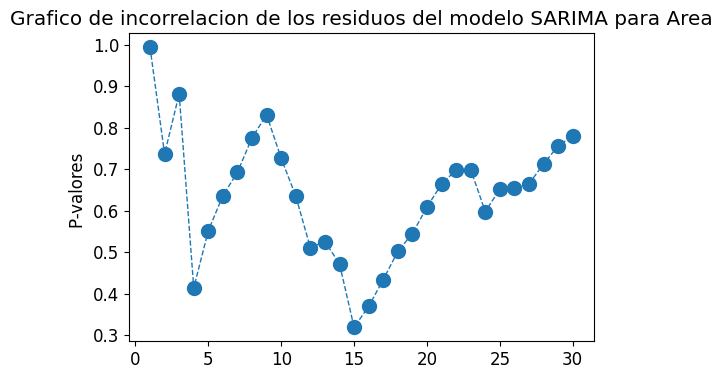
\includegraphics[scale=.52]{Figures/inco_area.png}
\caption{Área: gráfico de incorrelación (p--valores Ljung--Box por lag).}
\label{fig:inco_area}
\end{figure}

\begin{figure}[H]\centering
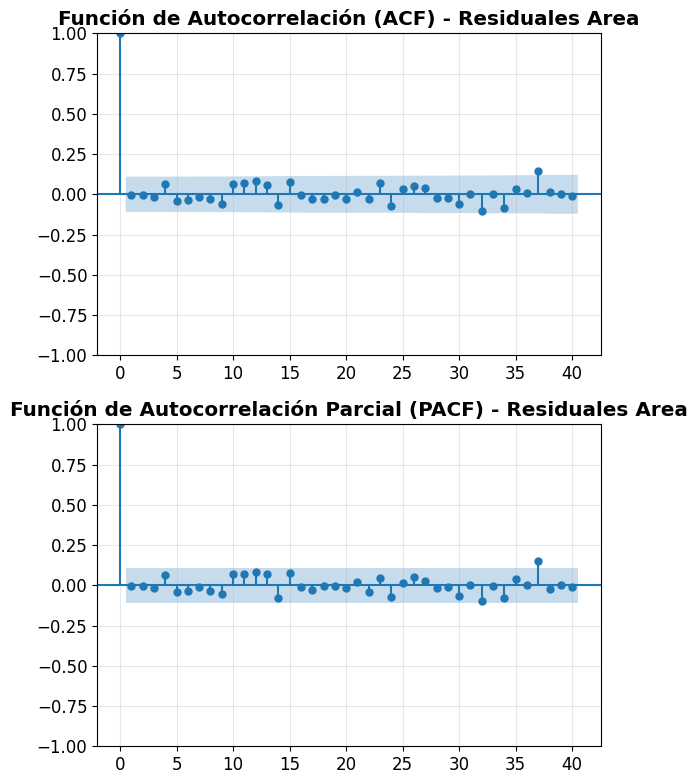
\includegraphics[scale=.52]{Figures/acf_pacf_res_area_d.png}
\caption{Área (diferenciada): ACF y PACF de los residuos.}
\label{fig:acf_pacf_res_area_d}
\end{figure}

\begin{figure}[H]\centering
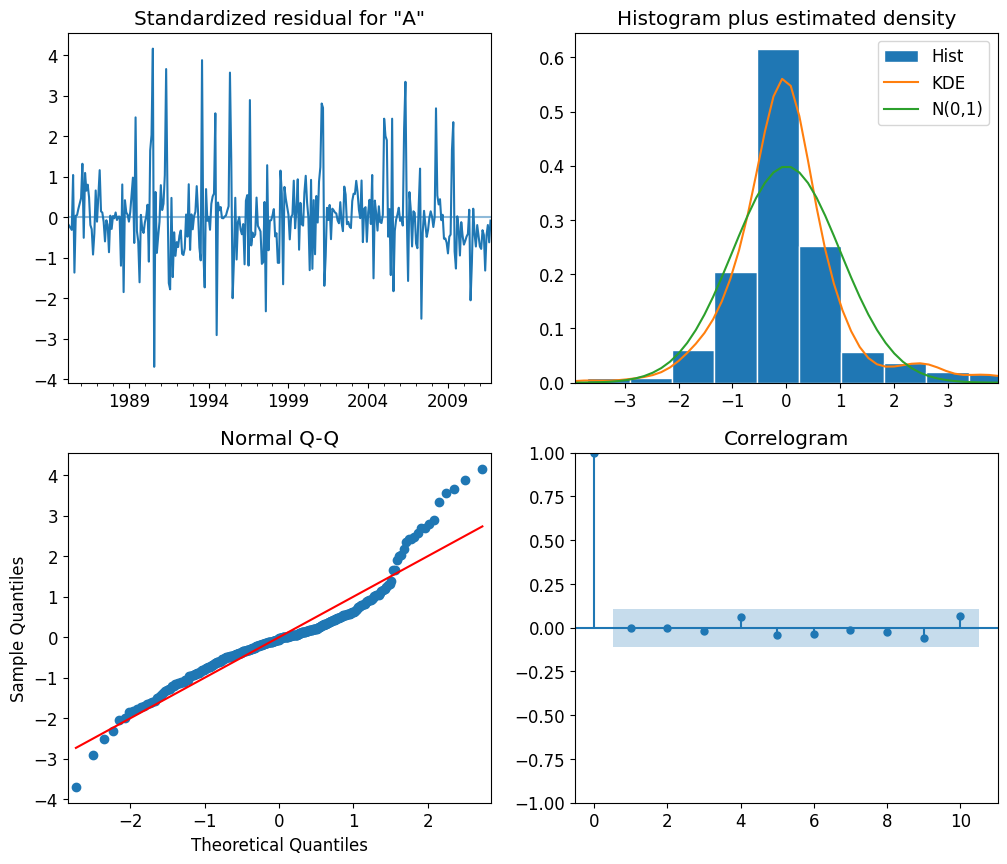
\includegraphics[scale=.52]{Figures/res_std_area_d.png}
\caption{Área (diferenciada): diagnóstico estándar de residuos (histograma, densidad, Q--Q, correlograma).}
\label{fig:std_area_d}
\end{figure}

\begin{figure}[H]\centering
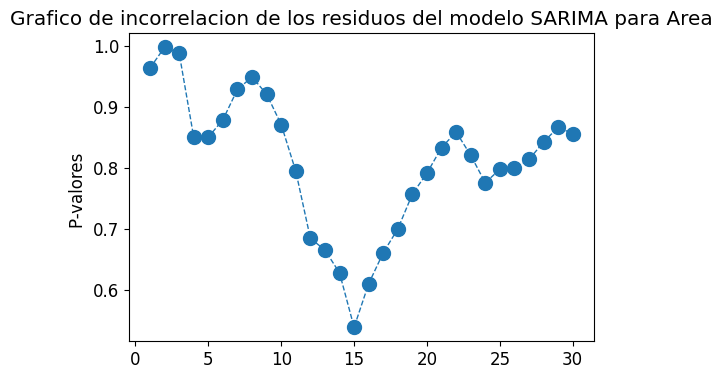
\includegraphics[scale=.52]{Figures/inco_area_d.png}
\caption{Área (diferenciada): gráfico de incorrelación (p--valores Ljung--Box por lag).}
\label{fig:inco_area_d}
\end{figure}